\chapter{Recuperação da Informação}
\label{cap:informationretrieval}

\begin{quotation}[]{Yoko Ono}
The computer is my favourite invention. I feel lucky to be part of the global village. I don't mean to brag, but I'm so fast with technology. People think it all seems too much, but we'll get used to it. I'm sure it all seemed too much when we were learning to walk.
\end{quotation}

A necessidade das pessoas de encontrar informação tem crescido bastante e tem se tornado uma prática de seu cotidiano. As informações devem ser precisas e estar disponíveis quase que imediatamente. Este capítulo fornece uma visão geral sobre Recuperação de Informação, a diferença entre recuperar uma informação e recuperar um dado e as técnicas utilizadas nas buscas.

\section{Introdução}

Nos tempos atuais, com o crescimento das bibliotecas virtuais e trocas eletrônicas de informações, há uma necessidade clara no melhoramento das técnicas de busca de informação. A gigantesca quantidade de informação e o tempo hábil do usuário para esperar por esses resultados são os fatores mais determinantes. 

Tendo como foco a melhoria na qual os dados são encontrados e celeridade em que são exibidas para o usuário, a indexação é uma das principais técnicas utilizadas em conjunto com outros algoritmos complexos \cite{Fred2008}.

Buscar informações, embora pareça uma atividade simples, é um processo muito impreciso. É esperado que o usuário possua uma noção vaga ao tentar buscar por uma informação, uma vez que não há uma interface direta que interprete exatamente às demandas do usuário e o resultado depende dos dados inicialmente fornecidos. Portanto, a interface deve ajudar o usuário na compreensão e expressão das necessidades de informação da melhor forma possível. Na formulação de suas consultas, fazendo a seleção da informação dentro de um conjunto de documentos, entendendo os resultados da pesquisa e acompanhar o progresso de suas buscas \cite{Baeza-Yates1999}.

\section{Recuperação de Informação versus Recuperação de Dados}

Uma série de características distinguem sistemas de Recuperação de Informação (\ac{RI}) de outras ferramentas de acesso à dados. Um sistema de \ac{RI} não extrai informações dos documentos acessados e normalmente também não processa as informações contidas nesses objetos. Isso separa os sistemas de RI de sistemas baseados no conhecimento, como sistemas especialistas. Essas ferramentas baseadas no conhecimento dependem fortemente de uma representação pré-definida de um domínio. Este conhecimento é geralmente utilizado para inferir, manipular ou categorizar informações através de dados. Diferente disso, os sistemas de Recuperação de Informação são usados para direcionar o usuário para documentos que possam ajudar a satisfazer suas necessidades de informação \citep{Ruthven2003}.

Recuperação de Dados (\ac{RD}) tem o propósito de encontrar dados que casam perfeitamente com a consulta, enquanto recuperação de informação visa encontrar os dados que possuam no mínimo alguma similaridade. Consequentemente, recuperação de dados é mais sensível à erros, considerando que um único documento errado retornando dentro de uma lista de outros milhares corretos, é uma falha total da busca. Por outro lado, recuperação de informação pode ser imprecisa e erros eventuais não compromete completamente o resultado da busca. Isso acontece porque recuperação de informação geralmente lida com textos semi-estruturados de linguagem natural, que pode ser semanticamente ambíguo enquanto recuperação de dados, procura por dados dentro de um ambiente estruturado, como por exemplo, um banco de dados relacional \cite{Fred2008}.

\begin{table}[htb]
	\centering
	\caption{Diferença entre sistemas \ac{RI} e \ac{RD}.}
	\label{tab:RIxRD}
	\begin{tabular}{|m{7cm} | m{2cm} | m{2cm} |}

		\hline
		
		\multicolumn{1}{|c|}{\bfseries Características / Métodos } & \multicolumn{1}{c|}{\bfseries RI} & \multicolumn{1}{c|}{\bfseries RD}\\ \hline
		Combinação exata   					&		&	x 	\\ \hline
		Alta sensibilidade a erros   			&		&	x  	\\ \hline
		Tratamento semântico   				&	x 	&	 	\\ \hline
		Busca em dados não estruturados   	&	x 	&	 	\\ \hline
		Inferência Dedutiva  					&		&	x  	\\ \hline
		Inferência Indutiva   					&	x 	&	 	\\ \hline
		Consulta de sintaxe controlada   		&		&	x 	\\ \hline
		Consulta com linguagem Natural   	&	x 	&	 	\\ \hline
		Mais utilizado em meios acadêmicos   &	x 	&	 	\\ \hline
		Comum em Produtos Comerciais   	&		&	x 	\\ \hline
		
	\end{tabular}
\end{table}

Ainda segundo \cite{Fred2008}, o usuário que utiliza um sistema de recuperação de informação não está apenas interessado naquela exata combinação de palavras. Geralmente essas palavras servem para que sistema possa encontrar um assunto no qual elas estão inseridas e muitas das vezes, documentos que possuam palavras sinônimas podem ser de interesse do usuário também. Já um usuário de um sistema de recuperação de dados, está buscando por um item específico, com características particulares e apenas itens que seja exatamente como descritos na busca, são de interesse do usuário. Qualquer outro resultado não satisfará a busca.

\section{Processamento de linguagem natural}
\subsection{Histórico}
\subsection{Sintática}
\subsection{Semântica}

\section{Estratégias de Recuperação}

De acordo com \cite{Grossman2004}, as estratégias de recuperação atribuem uma medida de similaridade entre uma consulta e um documento. Essas estratégias são baseadas na quantidade de ocorrências do termo em um documento. Quanto mais frequente o termo, mais relevante o documento. Além disso algumas dessas estratégias tratam das ambiguidades dos termos, e.g, \textit{rio de janeiro} e \textit{cidade maravilhosa}, podem ser referência ao mesmo conceito.
Os algoritmos consistem de uma consulta \textit{c} e um conjunto de documentos \textit{d\textsubscript{1}}, \textit{d\textsubscript{2}}, ..., \textit{d\textsubscript{n}} o coeficiente de similaridade é dado por \textit{SC(c,d\textsubscript{i})} para \textit{1 <= i <= n}.
Ainda de acordo com \cite{Grossman2004}, essas são algumas das estratégias que podem ser utilizadas:

\begin{itemize}
	\item{\textbf{Modelo vetorial}: Calcula a medida de similaridade através da definição de vetores que representam cada documento e um vetor que representa a consulta. Esse modelo é baseado na idéia que o significado de um documento é transmitido pelas palavras utilizadas. Se conseguir representar as palavras de um documento por um vetor, é possível comparar documentos e determinar o quão similar é o conteúdo.}
	
	\item{\textbf{Recuperação probabilística}: Consiste na probabilidade de que um termo irá aparecer em um documento relevante e é computada para cada termo em cada coleção. Para termos que coincidem entre a consulta e um documento, o coeficiente de similaridade é computado como a combinação das probabilidades de cada termo coincidente.}
	
	\item{\textbf{Modelos de linguagem}: Um modelo de linguagem estatística é um mecanismo probabilístico para “gerar” um texto. Ele define assim uma distribuição sobre todas as sequências de palavras possíveis. O modelo de linguagem mais simples é o modelo de linguagem do unigram, que é essencialmente uma distribuição de palavras.}
	
	\item{\textbf{Rede Bayesiana}: Uma rede Bayesiana é usada para inferir a relevância do documento para a consulta. Isso é baseado na “evidência” em um documento que permite inferir sobre a relevância do documento. A força dessa inferência é usada como o coeficiente de similaridade.}
	
	\item{\textbf{Boolean Indexing}: Uma pontuação é atribuída de tal forma que uma consulta booleana inicial resulta em uma classificação. Isso é feito associando um peso a cada termo de consulta para que esse peso seja usado para calcular o coeficiente de similaridade.}
	
	\item{\textbf{\ac{LSI}}: A ocorrência de termos em documentos é representada com uma matriz termo-documento. A matrix é decomposta através de decomposição em valores singulares (SVD) para filtrar os ruídos encontrados no documento, dessa forma, dois documentos que possuem a mesma semântica estão próximos um do outro num espaço multidimensional.}
	
	\item{\textbf{Redes Neurais}: A sequência de “neurônios”, ou nós em uma rede, que sinalizam quando ativados por uma consulta acionando links para documentos. A força de cada link na rede é transmitida para o documento e coletada para formar o coeficiente de singularidade entre a consulta e o documento. As redes são “treinadas” ajustando os pesos nos links em resposta para predeterminar documentos relevantes ou não.}
\end{itemize}


\section{Modelo Probabilístico de Recuperação}

Como brevemente abordado na seção anterior, o modelo de espaço vetorial calcula a medida de similaridade através da definição de vetores. O conteúdo de cada documento e os termos da consulta, conforme ilustrado na Figura \ref{fig:documento-vetor}, são traduzidos em vetores e dessa forma é possível medir a similaridade através de operações feitas em cima desses vetores. Os documentos cujo conteúdo, conforme medido através dos termos presentes no documento, correspondem mais ao conteúdo da consulta, são considerados os mais relevantes \citep{Grossman2004}.

\begin{figure}[htb]
	\centering
	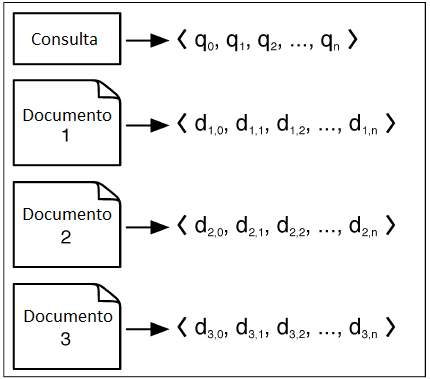
\includegraphics[scale=1.0]{chapters/informationretrieval/Document_as_Vectors.png}
	\caption{Representação dos vetores do modelo de espaço vetorial \citep{Grossman2004}.}
	\label{fig:documento-vetor}
\end{figure}

Este modelo envolve a construção de um vetor que representa os termos de um documento e outro vetor que representa os termos da pesquisa. Em seguida, um método de avaliação deve ser escolhido para medir o grau de aproximação de qualquer vetor documento com o vetor da consulta. Pode-se avaliar a diferença entre a magnitude entre dois vetores, mas geralmente isso prejudica documentos muito grandes e pode dar vantagem para documentos pequenos mas que não possuem muita similaridade \citep{Croft2010}.

Para continuar o entendimento sobre a similaridade desse modelo, é importante alguns conceitos sobre frequência de termos, frequência em documentos e frequência em coleção de documentos que serão abordados em seguida.

\subsection{Frequência de Termos}

De acordo com \cite{Manning2008}, um documento que menciona um termo da consulta mais frequentemente, pode ter uma relação maior com a consulta e, portanto, deveria receber uma pontuação maior. Veremos mais adiante que essa afirmação pode não ser verdade para todos os casos.

Tratando-se de frequência de termos bruta, atribuímos a cada termo de um documento um peso que depende do número de ocorrências do termo no documento. Gostaríamos calcular uma pontuação entre um termo da consulta \textit{t} e um documento \textit{d}, com base no peso de \textit{t} em \textit{d}. A abordagem mais simples é atribuir o peso igual ao número de ocorrências de um termo t num documento d. Este esquema de ponderação é referido como Frequência de Termos e é denotado por \textit{tf\textsubscript{t,d}} \citep{Manning2008}.

A ordem no qual os termos aparecem nos documentos não são levadas em consideração. O importante é apenas reter a frequência total dos termos da busca presentes em cada documento. Essa abordagem é conhecida na literatura como \textit{bag of word} \citep{Croft2010}.

\cite{Manning2008} esclarece ainda, que a frequência bruta não garante que um documento que possua um termo citado 20 vezes é mais relevante do que um documento que possui esse mesmo termo citado dez. Isso porque a relevância não aumenta linearmente proporcional à frequência de termos. Deste modo, frequência de termo logarítmica é mais interessante.

\begin{equation}
w_{t,d} = 
\left\{\begin{matrix}
 &1 +  \log_{10}tf_{t,d},  &se\ tf_{t,d} > 0 \\ 
 &0,  &caso\ contrario 
\end{matrix}\right.
\label{eq:log-tf}
\end{equation}

A tabela seguinte exibe um exemplificação da aplicação da frequência logarítmica de um mesmo termo presente em cinco documentos.

\begin{table}[H]
	\centering
	\caption{Exemplo de aplicação de frequência logarítmica de termos.}
	\label{tab:log-tf-table}
	\def\arraystretch{1.2} % padding da linhas da tabela
	\begin{tabular}{|m{3cm} | m{3cm} | m{3cm} |}

		\hline
		
		\multicolumn{1}{|c|}{\bfseries Documento } & \multicolumn{1}{c|}{\bfseries Frequência} & \multicolumn{1}{c|}{\bfseries Frequência log.}\\ \hline
		d1   					&	0		&	0 	\\ \hline
		d2   					&	1		&	1 	\\ \hline
		d3   					&	2		&	1,3 \\ \hline
		d4   					&	10		&	2	\\ \hline
		d5   					&	1000	&	4 	\\ \hline
		
	\end{tabular}
\end{table}

Como pode ser observado, ainda há importância na quantidade de ocorrência do termo, mas essa frequência não é mais tão determinante na relevância já que a frequência logarítmica aproxima os documentos.

\subsection{Frequência Inversa em Documentos}

 A utilização da frequência inversa em documentos vem da ideia de que termos mais raros são semanticamente mais informativos do que termos comuns. Termos comuns geralmente não possuem o poder de determinar o conteúdo de um documento, mas a presença de um termo raro em um documento aumenta a probabilidade deste documento ser estar fortemente relacionado à ele e, consequentemente, mais relevante para a busca \citep{Manning2008}.

Por exemplo, na área de Ciência da Computação, os termos \textit{código} e \textit{algoritmo} estão muito presentes nos mais diversos tipos de documentos. Se um usuário buscar por \textit{algoritmo de Dijkstra} e o sistema der importância igual aos dois termos e buscar por documentos que possuam apenas o termo \textit{algoritmo}, é improvável que esses documentos satisfaçam o usuário. Neste exemplo, o termo \textit{Dijkstra} tem o valor muito mais determinante na busca do que \textit{algoritmo} e, portanto, deve ter um peso maior na escolha dos documentos.

A definição trazida por \cite{Manning2008} diz que a frequência de documentos \textit{df\textsubscript{t}} corresponde ao total de documentos em uma coleção que contém o termo \textit{t} buscado. Disso, a frequência inversa em documentos, é a medida inversa da informatividade de um termo \textit{t}. Ou seja, quanto menor a frequência de documentos que no qual o termo \textit{t} está presente de uma dada coleção de documentos, mais informativo esses documentos devem ser. Essa fórmula é definida por:

\begin{equation}
idf = \log_{10}(N/df_{t})
\label{eq:idf}
\end{equation}

\subsection{TF–IDF}

Com essas duas medidas definidas acima, Frequência de Termos e Frequência Inversa em Documentos, pode-se aplicar \textit{tf-Idf weight} para determinar a importância do termo presente no documento com relação à coleção total de documentos. Em linhas gerais, tf-idf weight aumenta de acordo com o número de ocorrências de um termo e um documento e também aumenta de acordo com a raridade dos termos presentes no mesmo documento \cite{Manning2008}. 

Tf-idf possui três esquemas mas para simplificação e objetivo deste trabalho, abordaremos apenas a seguinte:
 
\begin{equation}
w_{t,d} = (1 + \log tf_{t,d}) \cdot \log_{10}(N/df_{t})
\label{eq:tf-idf}
\end{equation}

\subsection{Okapi BM25}

\section{Métodos de avaliação}
A partir das opções disponibilizadas para construir sistemas de recuperação da informação, resta buscar meios para os avaliar. Considerando que não existe método perfeito para todos os problemas é necessário se conduzir uma pesquisa para averiguar-se qual a melhor solução para determinado problema. Para fazer isso, determinam-se métricas que irão indicar se há conformidade da solução com o problema.

Uma das formas de se executar um experimento para avaliar o sistema é utilizar um conjunto de buscas e seus resultados esperados. A partir dessas buscas, avaliam-se as condições com que foram apresentados os resultados, levando em consideração desde o tempo que custou para achar essas informações até a quantidade de esforço necessária do usuário para encontrar uma informação relevante dentro do conjunto de resultados. Sendo estas as principais condições:
%As métricas mais relevantes podem variar de problema para problema, já que em alguns podemos ter algumas restrições que outros não possuam, como tempo, por exemplo
\begin{itemize}
    \item \textbf{Cobertura}. Representa o quanto de informações relevantes foram apresentadas como resultados. Considerando que para uma busca X existam 10 resultados relevantes, se apenas 3 foram apresentados para o usuário, temos uma cobertura de 30\%.
    \item \textbf{Ranking}. Métricas que utilizam o rank como parâmetro, avaliam o sistema de acordo com a posição dos itens relevantes nos resultados da busca. Um exemplo deste é o Mean Reciprocal Rank, onde para cada busca, a posição do primeiro documento relevante chamada K é usada pra determinar o Reciprocal Rank que é 1/K, em seguida, deve-se continuar executando mais N buscas onde encontraremos a média desses valores a partir de (1/K1 + 1/K2 + ... )/ N para encontrar o Mean Reciprocal Rank.
    \item \textbf{Precisão}. Informa o quanto de conteúdo relevante existe dentre os documentos apresentados. Por exemplo, se dentre 10 resultados retornados, apenas 2 resultados forem relevantes, temos uma precisão de 20\%.
    \item \textbf{Tempo de resposta}. É o intervalo médio entre o momento da consulta e a apresentação dos resultados.
    \item \textbf{Esforço do usuário}. Representa o esforço despendido pelo usuário para obter resultados em sua busca. Isso pode incluir diversos fatores que variam de acordo com a especificação do problema, sendo exemplos deles: número de linhas lida, número de ações necessárias para executar a busca, número de documentos abertos até encontrar o resultado desejado e outros.
\end{itemize}

\section{Tecnologias e Frameworks}

Para melhor lidar com os desafios de Recuperação da Informação, foram criadas novas tecnologias e frameworks. Essas tecnologias implementam os conceitos aqui utilizados e permitem modificações para que se adaptem melhor ao problema em questão. Os seguintes frameworks são os mais populares.

\begin{itemize}
    \item \textbf{Lucene}. O Apache Lucene é um motor de busca escrito em Java com ferramentas para busca em texto. É uma API open source disponível para download gratuito. Possui uma linguagem própria que permite fazer buscas parametrizadas com expressões regulares. 
    \item \textbf{Solr}. Solr é uma aplicação web construída ao redor do Lucene que adiciona funcionalidades como: busca geospacial, replicação, cacheamento e interfaces de administração.
    \item \textbf{Elasticsearch}. Assim como Solr, o Elasticsearch é uma aplicação construída com o uso do Lucene. O Elasticsearch é distribuído pela empresa Elastic e possui diversos plugins gratuitos e pagos para adicionar-se ferramentas de administração. Diferencia-se do Solr por focar mais em aspectos da administração do banco de dados e na escalabilidade.
\end{itemize}

\section{Sumário}

Foi abordado neste capítulo como e onde a Recuperação Informação é utilizada. Foi tratada a diferença entre Recuperação de Informação e Recuperação Dados e abordada algumas estratégias na recuperação de informações e como as avaliar. Houve um aprofundamento em modelos vetoriais, método que será usado neste trabalho.